\documentclass{beamer}
\usetheme{Madrid}

\usepackage{amsmath, amssymb, amsthm}
\usepackage{graphicx}
\usepackage{listings}
\usepackage{gensymb}
\usepackage[utf8]{inputenc}
\usepackage{hyperref}
\usepackage{gvv}
\usepackage{tikz}
\usetikzlibrary{decorations.pathmorphing}
\lstdefinestyle{CStyle}{
    language=C,
    basicstyle=\ttfamily\small,
    keywordstyle=\color{blue},
    stringstyle=\color{red},
    commentstyle=\color{green},
    showstringspaces=false,
    breaklines=true,
    frame=single,
    numbers=left,
    numberstyle=\tiny\color{gray}
}

\lstdefinestyle{PythonStyle}{
    language=Python,
    basicstyle=\ttfamily\small,
    keywordstyle=\color{blue},
    stringstyle=\color{red},
    commentstyle=\color{green},
    showstringspaces=false,
    breaklines=true,
    frame=single,
    numbers=left,
    numberstyle=\tiny\color{gray}
}



\begin{document}

\title{Question-1-1.11-11}
\author{EE24BTECH11035 - AKHIL}
\date{}
\frame{\titlepage}

\begin{frame}
\frametitle{Question}
The scalar product of the vector $\vec{a}=\hat{i}+\hat{j}+\hat{k}$ with a unit vector along the sum of the vector $\vec{b}=2\hat{i}+4\hat{j}-5\hat{k}$ and $\vec{c}=\lambda\hat{i}+2\hat{j}+3\hat{k}$ is equal to 1. Find the  value of $\lambda$ and hence find the  unit vector along $\Vec{b}+\Vec{c}$.\\
\end{frame}

\begin{frame}{allowframebreaks}
\frametitle{Inputs}

    \centering
    
    \label{tab:parameters}
	\begin{tabular}{ |c| c|}
    \hline
    \textbf{Point}  & \textbf{Coordinates}\\
    \hline
    $\vec{A}$ & $\myvec{1 \\ 1 \\1}$ \\
    \hline
    $\vec{B}$ & $\myvec{2 \\ 4 \\ -5}$\\
    \hline
\end{tabular}
\end{frame}

\begin{frame}
\frametitle{Solution}
Given vector $\vec{c}$ is:

\begin{align}
\vec{c} = \myvec{\lambda \\ 2 \\ 3}
\end{align}
The sum of vectors $\vec{b}$ and $\vec{c}$ is:
\begin{align}
\vec{b} + \vec{c} = \myvec{2 \\ 4 \\ -5} + \myvec{\lambda \\ 2 \\ 3} \\
= \myvec{2 + \lambda \\ 4 + 2 \\ -5 + 3} \\
= \myvec{2 + \lambda \\ 6 \\ -2}
\end{align}
\end{frame}

\begin{frame}
\frametitle{Solution}
Now, we find the norm of $\vec{b} + \vec{c}$. The norm is given by:

\begin{align}
\|\vec{b} + \vec{c}\| &= \sqrt{(\vec{b} + \vec{c})^\top (\vec{b} + \vec{c})} \\
&= \sqrt{(2 + \lambda)^2 + 6^2 + (-2)^2} \\
&= \sqrt{(2 + \lambda)^2 + 36 + 4} \\
&= \sqrt{(2 + \lambda)^2 + 40}
\end{align}

The unit vector along $\vec{b} + \vec{c}$ is:

\begin{align}
\hat{\vec{u}} &= \frac{\vec{b} + \vec{c}}{\|\vec{b} + \vec{c}\|}
\end{align}

\end{frame}

\begin{frame}
\frametitle{Solution}
Given,The scalar product of $\vec{a}$ with this unit vector as 1:

\begin{align}
\vec{a}^\top \hat{\vec{u}} &= 1
\end{align}

Substituting the expressions for $\vec{a}$ and $\hat{\vec{u}}$, we get:

\begin{align}
\begin{pmatrix} 1 & 1 & 1 \end{pmatrix} \cdot \frac{1}{\sqrt{(2 + \lambda)^2 + 40}} \myvec{2 + \lambda \\ 6 \\ -2} &= 1
\end{align}



\begin{align}
\frac{1}{\sqrt{(2 + \lambda)^2 + 40}} \left( (2 + \lambda) + 6 - 2 \right) &= 1 \\
\frac{1}{\sqrt{(2 + \lambda)^2 + 40}} ( \lambda + 6) &= 1
\end{align}

\end{frame}

\begin{frame}
\frametitle{Solution}
Squaring both sides:

\begin{align}
\frac{(\lambda + 6)^2}{(2 + \lambda)^2 + 40} &= 1
\end{align}



\begin{align}
(\lambda + 6)^2 &= (2 + \lambda)^2 + 40
\end{align}


\begin{align}
\lambda^2 + 12\lambda + 36 &= \lambda^2 + 4\lambda + 4 + 40
\end{align}
\end{frame}

\begin{frame}
\frametitle{solution}
Simplifying:

\begin{align}
12\lambda + 36 &= 4\lambda + 44 \\
8\lambda &= 8 \\
\lambda &= 1
\end{align}

Thus, $\lambda = 1$. Substituting $\lambda = 1$ into $\vec{b} + \vec{c}$:

\begin{align}
\vec{b} + \vec{c} &= \myvec{2 + 1 \\ 6 \\ -2} = \myvec{3 \\ 6 \\ -2}
\end{align}

The norm of $\vec{b} + \vec{c}$ is:

\begin{align}
\|\vec{b} + \vec{c}\| &= \sqrt{3^2 + 6^2 + (-2)^2} = \sqrt{9 + 36 + 4} = \sqrt{49} = 7
\end{align}
\end{frame}

\begin{frame}
\frametitle{solution}
Thus, the unit vector along $\vec{b} + \vec{c}$ is:

\begin{align}
\hat{\vec{u}} &= \frac{1}{7} \myvec{3 \\ 6 \\ -2} = \myvec{\frac{3}{7} \\ \frac{6}{7} \\ \frac{-2}{7}}
\end{align}
\end{frame}

\begin{frame}
\frametitle{Diagram}
\begin{figure}[h!]
	\centering
	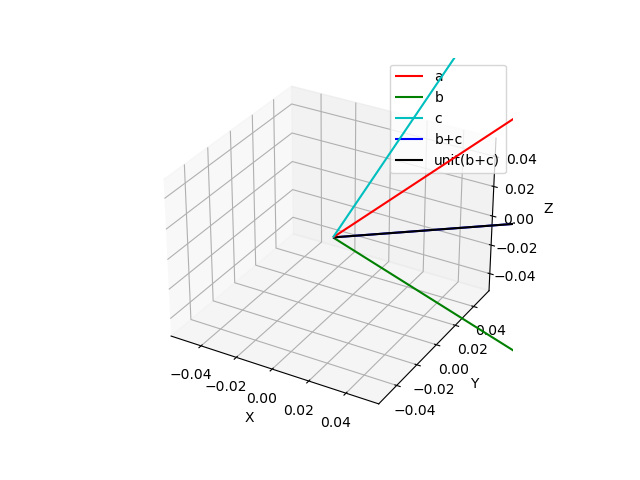
\includegraphics[width=0.5\linewidth]{figs/Figure_1.png}
	\caption{ $\vec{a},\vec{b},\vec{c}$,unit vector in the direction of  $\vec{b}+\vec{c}$}
	\label{stemplot}
\end{figure}	

\end{frame}
\begin{frame}[fragile]
\frametitle{Python code for graph}
\begin{lstlisting}[style=pythonstyle]
import numpy as np
import matplotlib.pyplot as plt

a = np.array([1, 1, 1])
b = np.array([2, 4, -5])
c = np.array([1, 2, 3])  # lambda = 1

b_plus_c = b + c

magnitude_b_plus_c = np.linalg.norm(b_plus_c)
unit_vector_b_plus_c = b_plus_c / magnitude_b_plus_c




\end{lstlisting}
\end{frame}
\begin{frame}[fragile]
\frametitle{Python code for graph}
\begin{lstlisting}[style=pythonstyle]
fig = plt.figure()
ax = fig.add_subplot(111, projection='3d')

ax.quiver(0, 0, 0, a[0], a[1], a[2], color='r', label='a')

ax.quiver(0, 0, 0, b[0], b[1], b[2], color='g', label='b')

ax.quiver(0, 0, 0, c[0], c[1], c[2], color='c', label='c')

ax.quiver(0, 0, 0, b_plus_c[0], b_plus_c[1], b_plus_c[2], color='b', label='b+c')


\end{lstlisting}
\end{frame}
\begin{frame}[fragile]
\frametitle{Python code for graph}
\begin{lstlisting}[style=pythonstyle]
# Plot the unit vector along b + c (black)
ax.quiver(0, 0, 0, unit_vector_b_plus_c[0], unit_vector_b_plus_c[1], unit_vector_b_plus_c[2], color='k', label='unit(b+c)')

# Set labels
ax.set_xlabel('X')
ax.set_ylabel('Y')
ax.set_zlabel('Z')
# Show legend
ax.legend()
# Show plot
plt.show()
\end{lstlisting}
\end{frame}
\begin{frame}[fragile]
\frametitle{C code for solution}
\begin{lstlisting}[style=Cstyle]
#include <stdio.h>
#include <stdlib.h>
#include <math.h>
#include "libs/matfun.h"
void printMatToFile(double **p, int m, int n, FILE *fp) {
    for (int i = 0; i < m; i++) {
        for (int j = 0; j < n; j++) {
            fprintf(fp, "%lf ", p[i][j]);
        }
        fprintf(fp, "\n");
    }
}

\end{lstlisting}
\end{frame}

\begin{frame}[fragile]
\frametitle{C code for solution}
\begin{lstlisting}[style=Cstyle]
   int main() {
    double lambda;
    double **a, **b, **c, **sum, **unitVec;
    double scalarProduct;
    FILE *outputFile = fopen("output.dat", "w");
    if (outputFile == NULL) {
        printf("Error opening file!\n");
        return 1;
    }
    a = createMat(3, 1);
    a[0][0] = 1;
    a[1][0] = 1;
    a[2][0] = 1;
   b = createMat(3, 1);
    b[0][0] = 2;
    b[1][0] = 4;
    b[2][0] = -5;
\end{lstlisting}
\end{frame}

\begin{frame}[fragile]
\frametitle{C code for solution}
\begin{lstlisting}[style=Cstyle]
 c = createMat(3, 1);
    for (lambda = -100; lambda <= 100; lambda += 0.01) {
        c[0][0] = lambda;
        c[1][0] = 2;
        c[2][0] = 3;
        sum = Matadd(b, c, 3, 1);
        unitVec = Matscale(sum, 3, 1, 1 / Matnorm(sum, 3));
       scalarProduct = Matdot(a, unitVec, 3);
        if (fabs(scalarProduct - 1.0) < 1e-6) {
            // Write the results to the output file
            fprintf(outputFile, "Found lambda = %lf\n", lambda);
            fprintf(outputFile, "Unit vector along b + c:\n");
            printMatToFile(unitVec, 3, 1, outputFile);
            break;
        }
    }

\end{lstlisting}
\end{frame}

\begin{frame}[fragile]
\frametitle{C code for solution}
\begin{lstlisting}[style=Cstyle]
        free(sum);
        free(unitVec);
    }

    free(a);
    free(b);
    free(c);
    fclose(outputFile);

    return 0;
}
\end{lstlisting}
\end{frame}
\end{document}

